%======================================================================
\chapter{Valence Bond Entanglement Entropy}
%======================================================================
\comment{SUPERNOTE: Make sure it's clear that I only did the VB EE part, not the DMRG/vN part.}

In \change{year that this happened} a new quantity called {\it{valence bond entanglement entropy}} ($\vb$) which seems to have properties
similar to entanglement entropy was proposed by \change{Fabian and co, also affleck or something?}.  
The main \change{draw, advantage} of this quantity is its \change{easy to measure -ableness,
ease of measurement?} when working in the valence bond basis.
For a valence bond basis state $\vb$ between two regions, A and B, is defined as 
\begin{equation}
\vb_A = \ln({2})\mathcal{N}_{\text{A}},
\end{equation} 
where $\mathcal{N}_{\text{A}}$ is the number of valence bonds crossing the boundary between
regions A and B.
\comment{Add in a figure showing this!!}


$\vb$ shares some properties with $\vn$; in particular, for both quantities: $S_{\text{A}} = S_{\text{B}}$.
Also, $\vb = 0$ for systems with no entanglement between regions A and B.
For any single valence bond basis state $\vb$ and $\vn$ agree exactly, and
in one-dimensional Heisenberg spin-1/2 systems, $\vb$ seems to to be in good agreement with
the conformal field theory (CFT) results for $\vn$.
However, in two dimensions $\vb$ shows a multiplicative logarithmic correction to the area law
for the isotropic Heisenberg model.  
Ground states of unfrustrated 2D spin-1/2 systems with exclusively nearest-neighbour interactions
are expected to follow an area law \comment {reference that paper (eisert)}, though for the 2D isotropic Heisenberg model the entanglement entropy had not yet been studied \change{explicitly}.


To \change{study/examine?} \change{this quantity} and check its \change{correspondence} to a known measure of entanglement we place our $\vb$ data alongside measurements of $\vn$
on the same system, calculated with density matrix renormalization group (DMRG) simulations. \comment{somehow say it wasn't done by me.} 
$\vb$ is calculated using valence bond quantum Monte Carlo (VB QMC) simulations.

\notsay{
In 1D we fit the entanglement entropy results to the analytical results from CFT...}
\comment{Do i do an overview of what i'm going to talk about in this part?}
%-----------------------------------------------------------------------------------------------------------------------
\section{One Dimensional Systems}
%-----------------------------------------------------------------------------------------------------------------------

\change{We begin by simulating one dimensional systems, examining both the cases of
open and periodic boundary conditions.}
The DMRG simulations require both of regions A and B to be topologically connected, and the 
same \change{convention} is used in the VB QMC simulations.

It is convenient to denote the size of region A by the number of sites included in that region 
(i.e. for a 1D system of length $L$, $S_{\text{A}} = S(x)$ is the entanglement entropy for a system where region A contains sites $\{1,2,\dots,x\}$ and the rest of the sites $\{x+1,x+2,\dots,L\}$
belong to region B.



\begin{figure} {
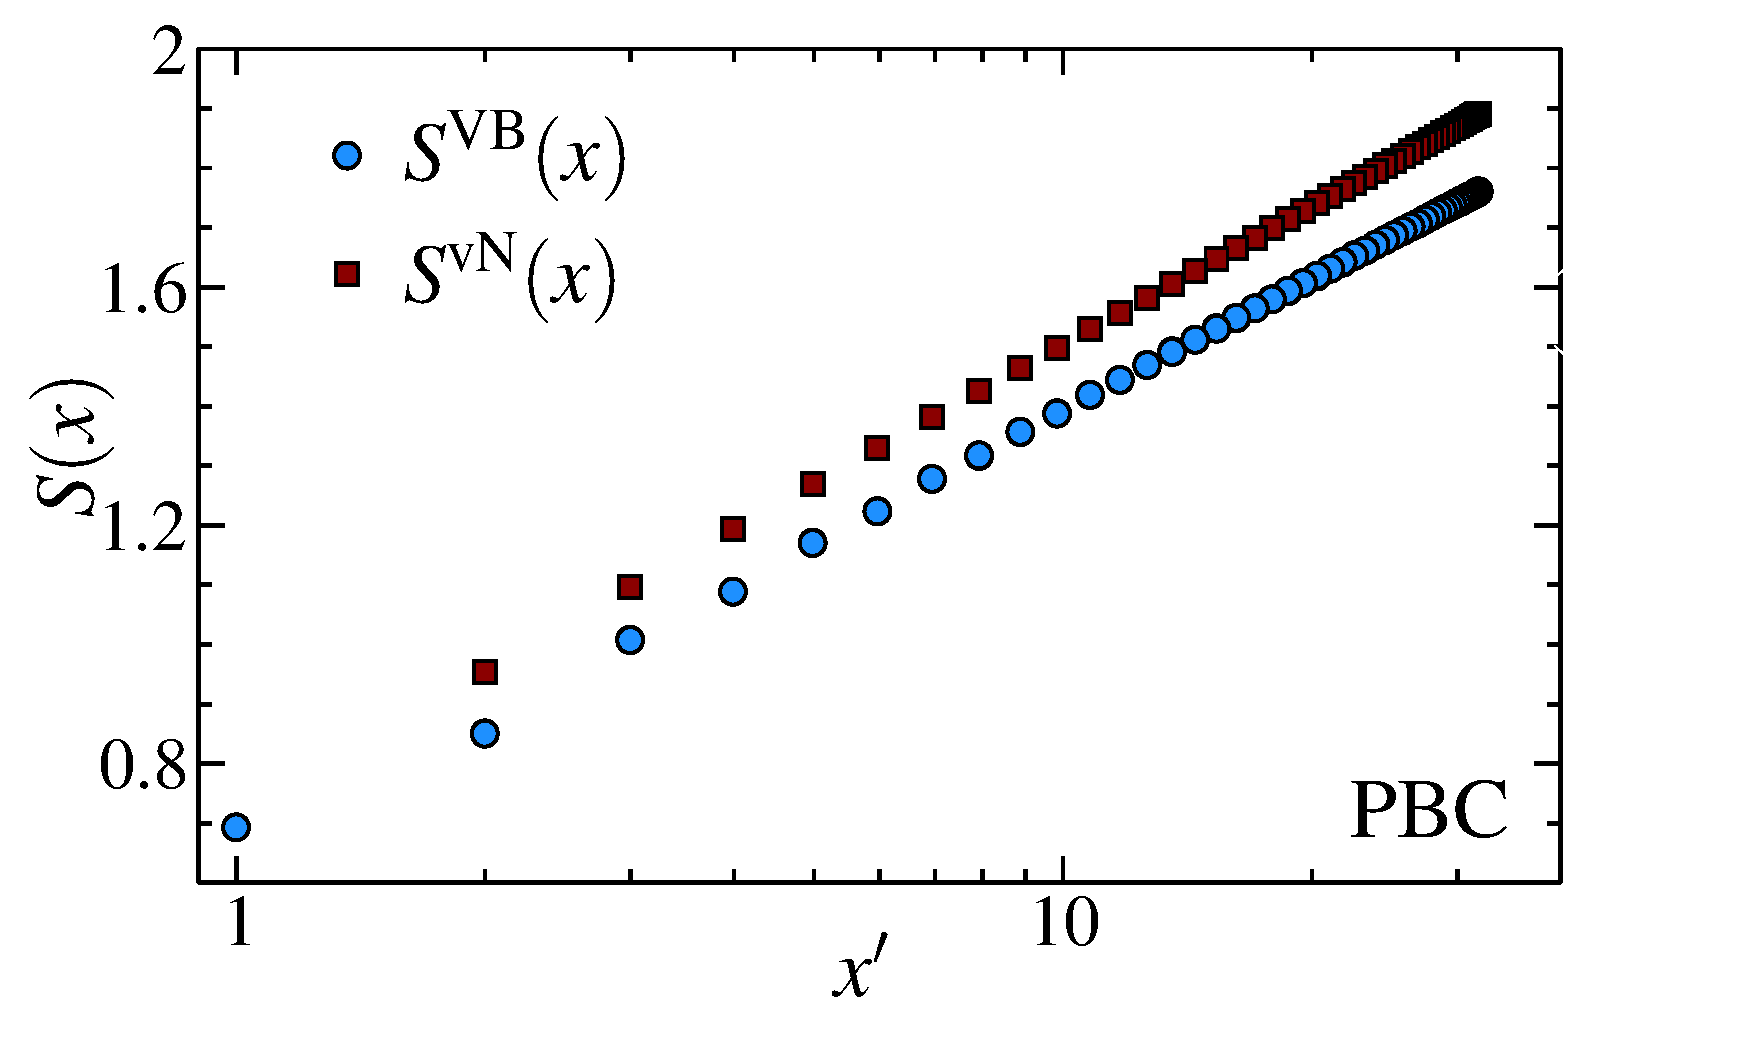
\includegraphics[width=4.5in]{./figures/paper1/figure1/thesis_pbc.eps} 
\centering
\caption[1D PBC Results for VB EE and von Neumann EE]{
{\color{red}
Entanglement entropies for a 1D Heisenberg chain with PBC and OBC. Upper
panels show the entropies as a function of the conformal distance $x'  = (L/\pi)\sin (\pi x/L)$ for
100-site chains.  Lower plots show the central
charge $c$, obtained by fitting the numerical data to the CFT result, for
several $L$.  For PBC, $c$ is calculated with the two smallest $x'$ points
removed.  For OBC, the fits depend on the number of sites included, $z$,
which we systematically decrease by removing $x'$ data points from the
{\it outside} ends of the chain.  $c$ is shown for $S^{\rm vN}$
(closed symbols) and $S^{\rm VB}$ (open symbols) for system sizes $L=64$
(circles), $L=100$ (squares), $L=128$ (diamonds), and $L=200$ (triangles)
\label{1dOBC}}
} }
\end{figure}

\begin{figure} {
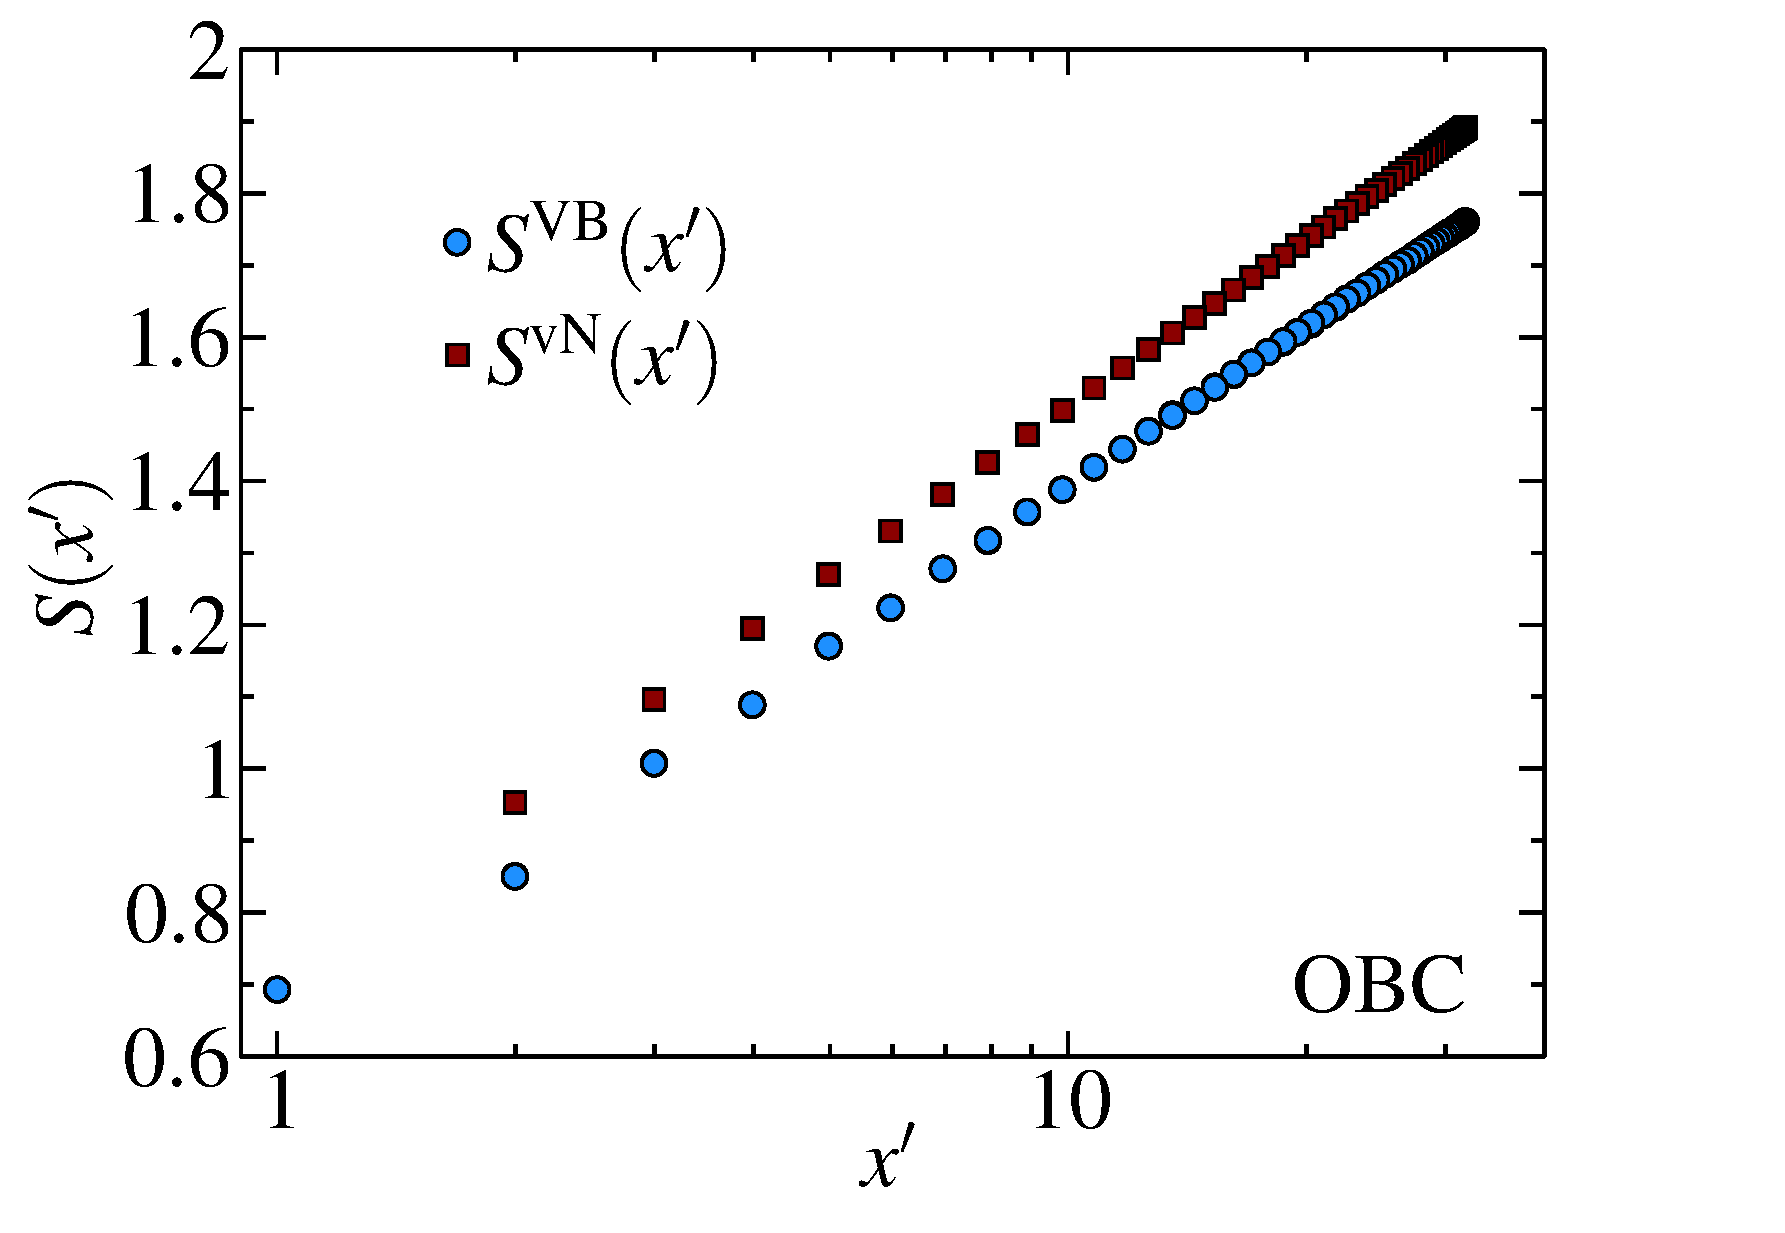
\includegraphics[width=4.5in]{./figures/paper1/figure1/thesis_obc.eps} 
\centering
\caption[1D OBC Results for VB EE and von Neumann EE]{
{\color{red}
Entanglement entropies for a 1D Heisenberg chain with PBC and OBC. Upper
panels show the entropies as a function of the conformal distance $x'  = (L/\pi)\sin (\pi x/L)$ for
100-site chains.  Lower plots show the central
charge $c$, obtained by fitting the numerical data to the CFT result, for
several $L$.  For PBC, $c$ is calculated with the two smallest $x'$ points
removed.  For OBC, the fits depend on the number of sites included, $z$,
which we systematically decrease by removing $x'$ data points from the
{\it outside} ends of the chain.  $c$ is shown for $S^{\rm vN}$
(closed symbols) and $S^{\rm VB}$ (open symbols) for system sizes $L=64$
(circles), $L=100$ (squares), $L=128$ (diamonds), and $L=200$ (triangles)
\label{1dOBC}}
} }
\end{figure}

\begin{figure} {

\includegraphics[width=6.5in]{./figures/paper1/figure1/4-panelFIG1.eps} 
\centering
\caption[1D Results for VB EE and von Neumann EE]{
{\color{red}
Entanglement entropies for a 1D Heisenberg chain with PBC and OBC. Upper
panels show the entropies as a function of the conformal distance $x'  = (L/\pi)\sin (\pi x/L)$ for
100-site chains.  Lower plots show the central
charge $c$, obtained by fitting the numerical data to the CFT result, for
several $L$.  For PBC, $c$ is calculated with the two smallest $x'$ points
removed.  For OBC, the fits depend on the number of sites included, $z$,
which we systematically decrease by removing $x'$ data points from the
{\it outside} ends of the chain.  $c$ is shown for $S^{\rm vN}$
(closed symbols) and $S^{\rm VB}$ (open symbols) for system sizes $L=64$
(circles), $L=100$ (squares), $L=128$ (diamonds), and $L=200$ (triangles)
\label{1D}}
} }
\end{figure}



\section{Approaching Two Dimensions}

\begin{figure} { 
\includegraphics[width=6.5in]{./figures/paper1/figure23new/fig23NEW.eps}
\caption[EEs for 3- \& 4-leg ladders]{
{\color{red}
Entanglement entropies for 3-leg (left)
and 4-leg (right) ladder systems with OBC and 100 sites per leg.  For
odd-leg ladders, $S(x)\propto\ln(x')$.  The left
inset shows $S(x)$ as a function of the conformal distance, $x'$, on a log
scale. For even-leg ladders, $S(x\gtrsim\xi)= {\rm const}.$
The right inset shows the site indexing used for multi-leg ladders where the
bipartition A is shaded and labeled by $x=9$. 
}
 \label{ladder} }} 
 \end{figure}

\section{The Area Law}

\begin{figure} { \includegraphics[width=6.5in]{./figures/paper1/figure4/fig4.eps}
 \caption[Area Law in 2D Heis model]{
 {\color{red} Entanglement entropies divided by $N$,  for $N$-leg Heisenberg
(filled symbols) and free-fermion (open diamonds) ladders, taken such that
the region A includes $2N^2$ sites.  
For the Heisenberg model and large $N$, $S^{\rm VB}\propto N \ln N$,
whereas $S^{\rm vN}\propto N$.  
Data for free fermions, $S^{\rm vN}_{\rm ff}\propto N \ln N$,  are shown for comparison.
We show data for ladders with length (sites per leg) $L =100$ and
%ladders with length proportional to the number of legs 
$L=4N$.  
}
\label{zigzag}}} 
\end{figure}
